
\documentclass[11pt,twocolumn]{article}

\usepackage[margin=0.6in]{geometry}
\setlength{\columnsep}{0.3in}
\usepackage{amsmath}
\usepackage{booktabs}
\usepackage{graphicx}
\usepackage{parskip}
\usepackage{titlesec}
\titlespacing*{\section}{0pt}{10pt plus 2pt minus 2pt}{5pt}
\titlespacing*{\subsection}{0pt}{8pt plus 2pt minus 2pt}{4pt}
\usepackage{float}
\usepackage{caption}
\captionsetup{skip=4pt}
\setlength{\intextsep}{8pt}
\setlength{\textfloatsep}{10pt}
\usepackage{tikz}
\usetikzlibrary{arrows.meta,calc}
\usepackage{pgfplots}
\pgfplotsset{compat=1.18}

\title{Dynamics Lab}
\author{A. Student}
\date{November 2, 2026}

\begin{document}
\raggedbottom
\maketitle

\section{Question}

Does the relationship between net force and acceleration of a cart on an inclined track obey Newton's Second Law?

\section{Hypothesis}

Our hypothesis is that the relationship between net force and acceleration will be linear. Because of that, the slope ($\frac{F}{a}$) of the graph of net force vs.\ acceleration will equal the total mass of the system.

\section{Strategy}

Our setup used a cart with a mass of $m_3$ on an inclined track connected over two pulleys to hanging masses $m_1$ and $m_2$ respectively. The height and horizontal length of a section of the ramp were measured to calculate its incline angle ($\theta$). During each round, a 20g mass was removed from $m_1$ and added to $m_2$ while keeping the \textit{total} mass constant. A motion sensor in the cart recorded its acceleration. The measurements were averaged, and the calculated net force was graphed against acceleration to compare the slope with the total mass of the system.

\begin{figure}[H]
  \centering
  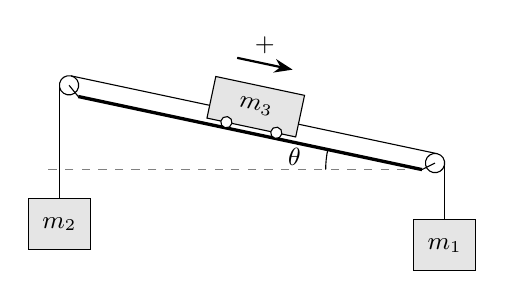
\begin{tikzpicture}[scale=0.72, >=Stealth]
  \begin{scope}[xscale=-1]
    \draw[dashed, gray] (0,0) -- (6.6,0);
    \draw (1.7,0) arc (0:12:1.7);
    \node at (2.25,0.22) {\small $\theta$};
    \begin{scope}[rotate=12]
      \draw[very thick] (0,0) -- (6.2,0);
      \draw (-0.2,0.16) circle (0.17);
      \draw (6.4,0.16) circle (0.17);
      \draw (0,0) -- (-0.2,0.16);
      \draw (6.2,0) -- (6.4,0.16);
      \coordinate (C1) at (-0.2,0.16);
      \coordinate (C2) at (6.4,0.16);
      \draw[fill=gray!20] (2.3,0.1) rectangle (3.9,0.85);
      \draw[fill=white] (2.65,0.1) circle (0.1);
      \draw[fill=white] (3.55,0.1) circle (0.1);
      \node[rotate=-12, inner sep=0] at (3.1,0.48) {\small $m_3$};
      \draw (2.3,0.33) -- (-0.2,0.33);
      \draw (3.9,0.33) -- (6.4,0.33);
      \draw[->, thick] (3.6,1.25) -- (2.6,1.25);
      \node[above] at (3.1,1.25) {\small $+$};
    \end{scope}
    \draw (C1) ++(-0.17,0) -- ++(0,-1.0) coordinate (H1);
    \draw[fill=gray!20] (H1) ++(-0.55,0) rectangle ++(1.1,-0.9);
    \node at ($(H1)+(0,-0.45)$) {\small $m_1$};
    \draw (C2) ++(0.17,0) -- ++(0,-2.0) coordinate (H2);
    \draw[fill=gray!20] (H2) ++(-0.55,0) rectangle ++(1.1,-0.9);
    \node at ($(H2)+(0,-0.45)$) {\small $m_2$};
  \end{scope}
  \end{tikzpicture}
  \caption{Experimental setup. Positive motion is toward $m_1$.}
\end{figure}

\section{Data}

We measured the cart to be $0.2942\ \text{kg}$.

At the section of the ramp that we measured, the vertical height was $6.80\ \text{cm}$ and the horizontal length was $74.95\ \text{cm}$.

\begin{table}[H]
  \centering
  \footnotesize
  \setlength{\tabcolsep}{1.8pt}
  \begin{tabular}{ccccccc}
    \toprule
    Round & $m_1$ (g) & $m_2$ (g) & $a_1$ & $a_2$ & $a_3$ & $a_{\text{avg}}$ \\
    \midrule
    1 & 110 & 50  & 1.662    & 1.688      & --      & 1.675    \\
    2 & 90  & 70  & 0.8886   & 0.7794*    & 0.8658  & 0.8772   \\
    3 & 70  & 90  & 0.05836  & 0.06267    & --      & 0.06052  \\
    4 & 50  & 110 & $-0.7215$ & $-0.3488$* & $-0.7213$ & $-0.7214$ \\
    \bottomrule
  \end{tabular}
  \caption{Measured acceleration (m/s$^2$). Asterisks mark excluded outliers.}
\end{table}

One trial in Round 2 and one trial in Round 4 were excluded as outliers because they were substantially different from the other measurements in their respective rounds. Because of this, we did a third trial for Round 1 and Round 4 to get an accurate measurement.

\section{Analysis}

\subsection{Free Body Diagrams}

\begin{figure*}[t]
  \centering
  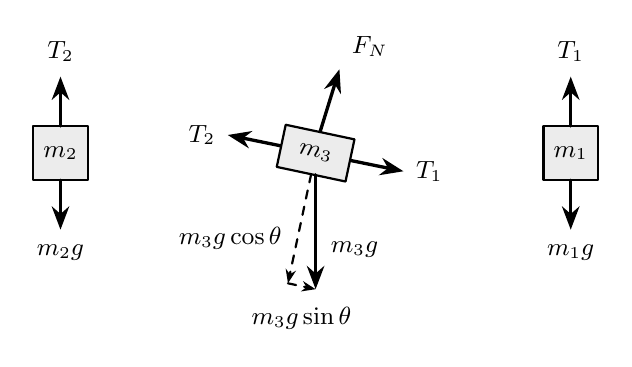
\begin{tikzpicture}[
    scale=0.72, every node/.style={font=\small},
    >=Stealth,
    line cap=round,
    line join=round,
    force/.style={->, very thick},
    component/.style={->, thick, dashed}
  ]

    \begin{scope}[shift={(0,0)}]
      \draw[fill=gray!15, thick]
        (-0.48,-0.48) rectangle (0.48,0.48);
      \node at (0,0) {$m_2$};
      \draw[force] (0,0.48) -- (0,1.35);
      \node[above=2pt] at (0,1.35) {$T_2$};
      \draw[force] (0,-0.48) -- (0,-1.35);
      \node[below=2pt] at (0,-1.35) {$m_2g$};
    \end{scope}

    \begin{scope}[shift={(4.5,0)}]
      \begin{scope}[rotate=-12]
        \draw[fill=gray!15, thick]
          (-0.62,-0.38) rectangle (0.62,0.38);
        \node[rotate=-12] at (0,0) {$m_3$};
      \end{scope}
      \draw[force] (-0.62,0.13) -- (-1.55,0.32);
      \node[left=1pt] at (-1.55,0.32) {$T_2$};
      \draw[force] (0.62,-0.13) -- (1.55,-0.32);
      \node[right=1pt] at (1.55,-0.32) {$T_1$};
      \draw[force] (0.08,0.38) -- (0.42,1.48);
      \node[above right=1pt] at (0.42,1.48) {$F_N$};
      \draw[force] (0,-0.38) -- (0,-2.4);
      \node[right=2pt] at (0,-1.7) {$m_3g$};
      \draw[component, -{Stealth[length=5pt]}] (-0.079,-0.372) -- (-0.488,-2.296);
      \node[left=2pt] at (-0.33,-1.5) {$m_3g\cos\theta$};
      \draw[component, -{Stealth[length=5pt]}] (-0.488,-2.296) -- (0,-2.4);
      \node[below=4pt] at (-0.25,-2.35) {$m_3g\sin\theta$};
    \end{scope}

    \begin{scope}[shift={(9,0)}]
      \draw[fill=gray!15, thick]
        (-0.48,-0.48) rectangle (0.48,0.48);
      \node at (0,0) {$m_1$};
      \draw[force] (0,0.48) -- (0,1.35);
      \node[above=2pt] at (0,1.35) {$T_1$};
      \draw[force] (0,-0.48) -- (0,-1.35);
      \node[below=2pt] at (0,-1.35) {$m_1g$};
    \end{scope}

  \end{tikzpicture}
  \caption{Free body diagrams for the two hanging masses and the cart.}
\end{figure*}

The free body diagrams show the forces acting on each object. For the cart, gravity is split into two parts, one parallel to the incline and one perpendicular to it.

Taking positive motion as down the incline for the cart, down for $m_1$, and up for $m_2$, by adding all parts of the total system, Newton's Second Law ($\sum F=ma$), gives the following result.
\begin{align*}
m_1g-T_1 &= m_1a,\\
T_1-T_2+m_3g\sin\theta &= m_3a,\\
T_2-m_2g &= m_2a.
\end{align*}

Adding the equations cancels both tensions:
\[
\begin{aligned}
&(m_1g-T_1)+(T_1-T_2+m_3g\sin\theta)\\
&\qquad +(T_2-m_2g)=(m_1+m_2+m_3)a,
\end{aligned}
\]
so
\[
m_1g-m_2g+m_3g\sin\theta=(m_1+m_2+m_3)a.
\]

The left side is the net force, $F$. With constant total mass, $F$ \textit{should} be proportional to $a$, so $F$ was graphed against $a$.

\subsection{Angle of the Incline}

The ramp measurements form a right triangle. The height is opposite the incline angle and the horizontal length is adjacent, so
\[
\theta=\tan^{-1}\!\left(\frac{6.80}{74.95}\right)=5.18^\circ.
\]

\subsection{Graphs}

The average acceleration for Round 1 was
\[
a=\frac{1.662+1.688}{2}=1.675\ \text{m/s}^2.
\]

Using $g=9.8\ \text{m/s}^2$, its net force was
\begin{align*}
F&=(0.110)(9.8)-(0.050)(9.8)\\
&\quad +(0.2942)(9.8)\sin(5.18^\circ)=0.849\ \text{N}.
\end{align*}

This gives the point $(1.675,0.849)$. The same calculation was performed for each round and a linear trendline was fitted to the data using Excel.

\begin{figure}[H]
  \centering
  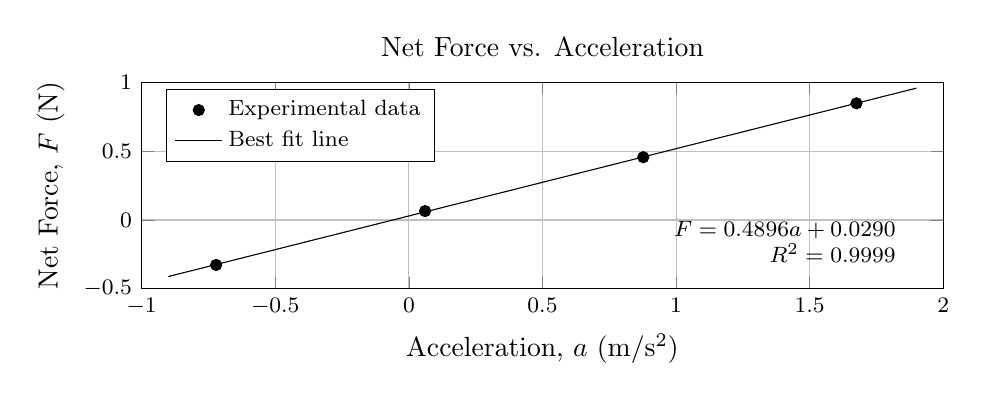
\begin{tikzpicture}
    \begin{axis}[
      width=0.97\linewidth, height=4.2cm,
      title={Net Force vs. Acceleration},
      xlabel={Acceleration, $a$ (m/s$^2$)},
      ylabel={Net Force, $F$ (N)},
      grid=both,
      xmin=-1, xmax=2,
      ymin=-0.5, ymax=1,
      legend pos=north west,
      legend cell align=left,
      legend style={font=\footnotesize},
      tick label style={font=\footnotesize},
    ]
      \addplot[only marks, mark=*] coordinates {
        (1.675, 0.8485) (0.8772, 0.4565)
        (0.06052, 0.0645) (-0.7214, -0.3275)
      };
      \addlegendentry{Experimental data}

      \addplot[domain=-0.9:1.9, black] {0.4896*x + 0.0290};
      \addlegendentry{Best fit line}

      \node[anchor=south east, font=\footnotesize]
        at (rel axis cs:0.97,0.04)
        {$\begin{array}{r}F = 0.4896a + 0.0290\\ R^2 = 0.9999\end{array}$};
    \end{axis}
  \end{tikzpicture}
  \caption{Net force versus acceleration.}
\end{figure}

\subsection{Calculations}

The best fit equation, given by Excel, is $F=(\textbf{0.4896})a+0.0290\ \text{N}$. Additionally, further analysis using Excel found $R^2=0.9999$. The slope ($\frac{F}{a}$) gives the experimental mass. The small nonzero intercept suggests that some other error may have affected the measurements.

\[
\boxed{m_{\text{experimental}}=0.4896\ \text{kg}}
\]

\section{Conclusion}

\subsection{Evaluation of Results}

The expected total mass is
\[
m_{\text{expected}}=0.110+0.050+0.2942=0.4542\ \text{kg}.
\]

The percent error is
\[
\frac{|0.4896-0.4542|}{0.4542}\times100\%=\boxed{7.8\%}.
\]

Based on the evaluations, the experimental mass was slightly larger than the expected mass. However, the data still stuck to a linear trend ($R^2=0.9999$), and the experimental slope was reasonably close to the expected total mass, with a percent error of 7.8\%. Therefore, these results support our initial hypothesis that net force and acceleration have a linear relationship.

\subsection{Sources of Error}

When coming to potential sources of error, there are two obvious possibilities. First, friction between the wheels of the cart and the ramp could have decreased the measured acceleration and henceforth affected the results. Second, the pulleys had rotational inertia that was not accounted for in the calculated total mass of the cart and hanging weights, which could have also affected the results.

\end{document}
